\documentclass[final,t]{beamer}
\mode<presentation>
{
%  \usetheme{Warsaw}
%  \usetheme{Aachen}
%  \usetheme{Oldi6}
%  \usetheme{I6td}
  \usetheme{I6dv}
%  \usetheme{I6pd}
%  \usetheme{I6pd2}
}
% additional settings
\setbeamerfont{itemize}{size=\normalsize}
\setbeamerfont{itemize/enumerate body}{size=\normalsize}
\setbeamerfont{itemize/enumerate subbody}{size=\normalsize}
% additional packages
\usepackage{ragged2e}
\usepackage{verbatim}
\usepackage{textcomp}
\usepackage[ampersand]{easylist}
\usepackage{lipsum}
\usepackage{times}
\usepackage{amsmath,amsthm, amssymb, latexsym}
\usepackage{exscale}
%\boldmath
\usepackage{booktabs, array}
%\usepackage{rotating} %sideways environment
\usepackage[english]{babel}
\usepackage[latin1]{inputenc}
\usepackage[orientation=landscape,size=custom,width=111.76,height=86.36,scale=1]{beamerposter}
\addtobeamertemplate{block begin}{}{\justifying}
\usepackage[export]{adjustbox}
\listfiles
\graphicspath{{figures/}}
% Display a grid to help align images
%\beamertemplategridbackground[1cm]

\title{\huge YAX: Taxonomic assignment using metagenomic shotgun sequences}
\author{Evan T. Bolyen$^{a}$, Mike R. DeBerg$^{a}$, Andrew J. Hodel$^{a}$, Hayden T. Westbrook$^{a}$, and Viacheslav Y. Fofanov$^{a}$}
\institute{$^{a}$School of Informatics, Computing, and Cyber Systems - Northern Arizona University}

% abbreviations
\usepackage{xspace}
\makeatletter
\DeclareRobustCommand\onedot{\futurelet\@let@token\@onedot}
\def\@onedot{\ifx\@let@token.\else.\null\fi\xspace}
\def\eg{{e.g}\onedot} \def\Eg{{E.g}\onedot}
\def\ie{{i.e}\onedot} \def\Ie{{I.e}\onedot}
\def\cf{{c.f}\onedot} \def\Cf{{C.f}\onedot}
\def\etc{{etc}\onedot}
\def\vs{{vs}\onedot}
\def\wrt{w.r.t\onedot}
\def\dof{d.o.f\onedot}
\def\etal{{et al}\onedot}
\makeatother

%%%%%%%%%%%%%%%%%%%%%%%%%%%%%%%%%%%%%%%%%%%%%%%%%%%%%%%%%%%%%%%%%%%%%%%%%%%%%%%%%%%%%%%%%%%%%%%%%%%%%%%%%%%%
%%%%%%%%%%%%%%%%%%%%%%%%%%%%%%%%%%%%%%%%%%%%%%%%%%%%%%%%%%%%%%%%%%%%%%%%%%%%%%%%%%%%%%%%%%%%%%%%%%%%%%%%%%%%
\begin{document}
\begin{frame}{}
  \begin{columns}[t]
    \begin{column}{.3\linewidth}
        \begin{alertblock}{
\includegraphics[width=.8\linewidth]{assets/yak}\newline\newline}
            YAX is a both a tool for taxonomic classification and a computational pipeline manager.\newline
        \end{alertblock}
        \begin{block}{Purpose}
            To seek out new life and new civilizations and to boldly go where no man has gone before. To provide a dynamic taxonomic assignment pipeline.
            % YAX is ultimately a pipeline used for taxonomic assignment of a set of sample sequences. However it is designed to
            % be dynamic in a way that allows for not only parameter exploration with as little recomputation as possible but also
            % for modification of the pipeline itself with as little effor as possible. This makes YAX capable of rapid recalculations
            % and reconfigurations.
        \end{block}
        \begin{block}{Requirements}
            \textbf{Modular}
            \begin{itemize}
                \item[$\bullet$]Incorporate developing technologies
                \item[$\bullet$]Evaluate different processes
            \end{itemize}
            \vspace{0.5cm}
            \textbf{Fail Early}
            \begin{itemize}
                \item[$\bullet$]Validate parameters and dependencies before running
                \item[$\bullet$]Prevent failure in the middle of a run for spurious reasons
            \end{itemize}
            \vspace{0.5cm}
            \textbf{Coverage Representation}
            \begin{itemize}
                \item[$\bullet$]Provide biologists with relevant details
                \item[$\bullet$]Every identified taxon is qualified with coverage data
            \end{itemize}
            \vspace{0.5cm}
            \textbf{State System}
            \begin{itemize}
                \item[$\bullet$]Manage component requirements
                \item[$\bullet$]Control and record all data produced
                \item[$\bullet$]Eliminates redundant recomputation
                \item[$\bullet$]Allows parameter exploration
            \end{itemize}
        \end{block}

        \begin{block}{Managing State}
            The figure below represents multiple runs of a pipeline. By using a state-system, YAX is able to identify where parameters are shared and reuse the results. \\
            \includegraphics[width=1\linewidth]{assets/Artifacts}
        \end{block}

      %%%%%%%%%%%%%%%%%%%%%%%%%%%%%%%%%%%%%%%%%%%%%%%%%%%%%%%%%%%%%%%%%%%%%%%%%%%%%%%%%%%%%%%%%%%%%%%%%%%%%%%%%%%%


    \end{column}
    \begin{column}{.3\linewidth}
        %%%%%%%%%%%%%%%%%%%%%%%%%%%%%%%%%%%%%%%%%%%%%%%%%%%%%%%%%%%%%%%%%%%%%%%%%%%%%%%%%%%%%%%%%%%%%%%%%%%%%%%%%%%%


        \begin{block}{Assigning Taxonomy}
            \textbf{Use strict matching against the entire reference set to remove obviously wrong results:}\\
            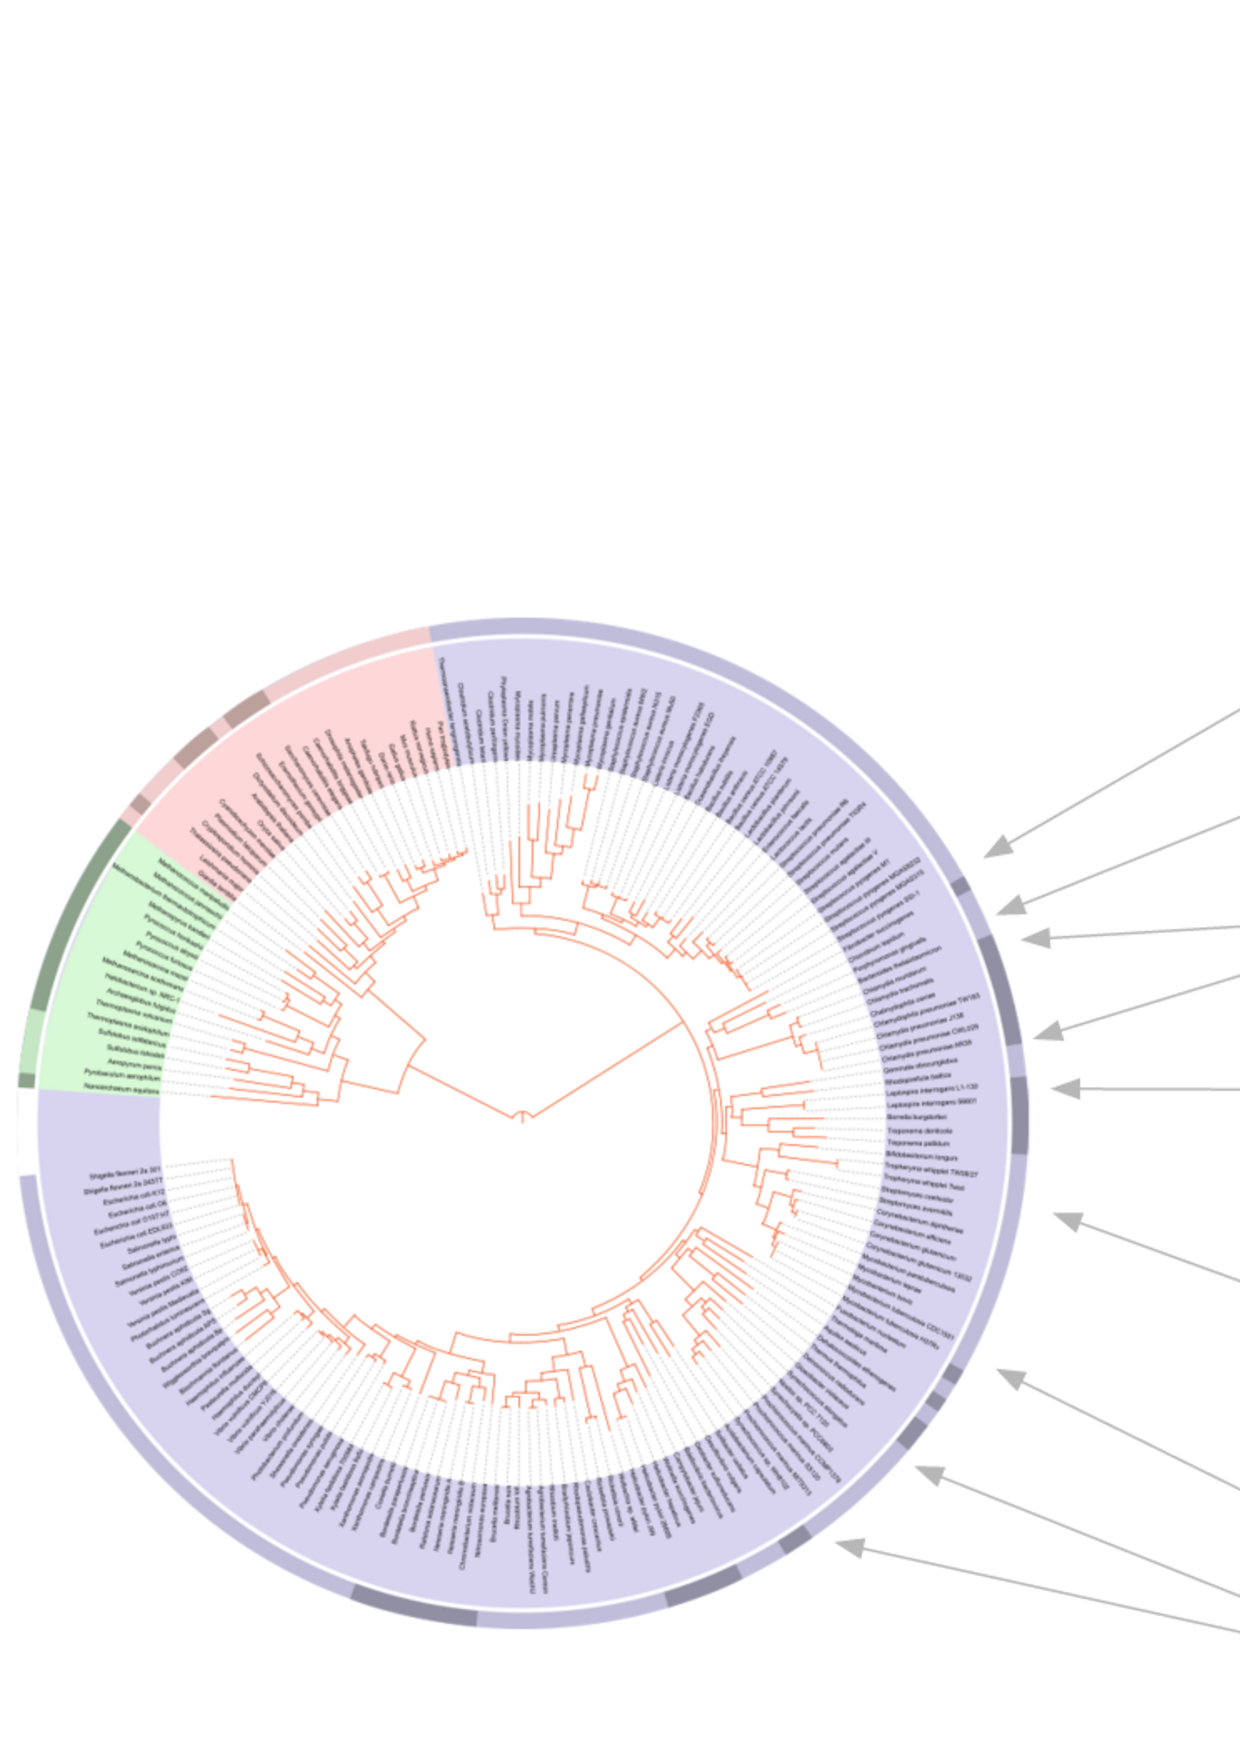
\includegraphics[width=.8\linewidth, right]{assets/Whole} \\
            \textbf{Using the results from the last step, perform a detailed\\ refinement with looser parameters:}\\
            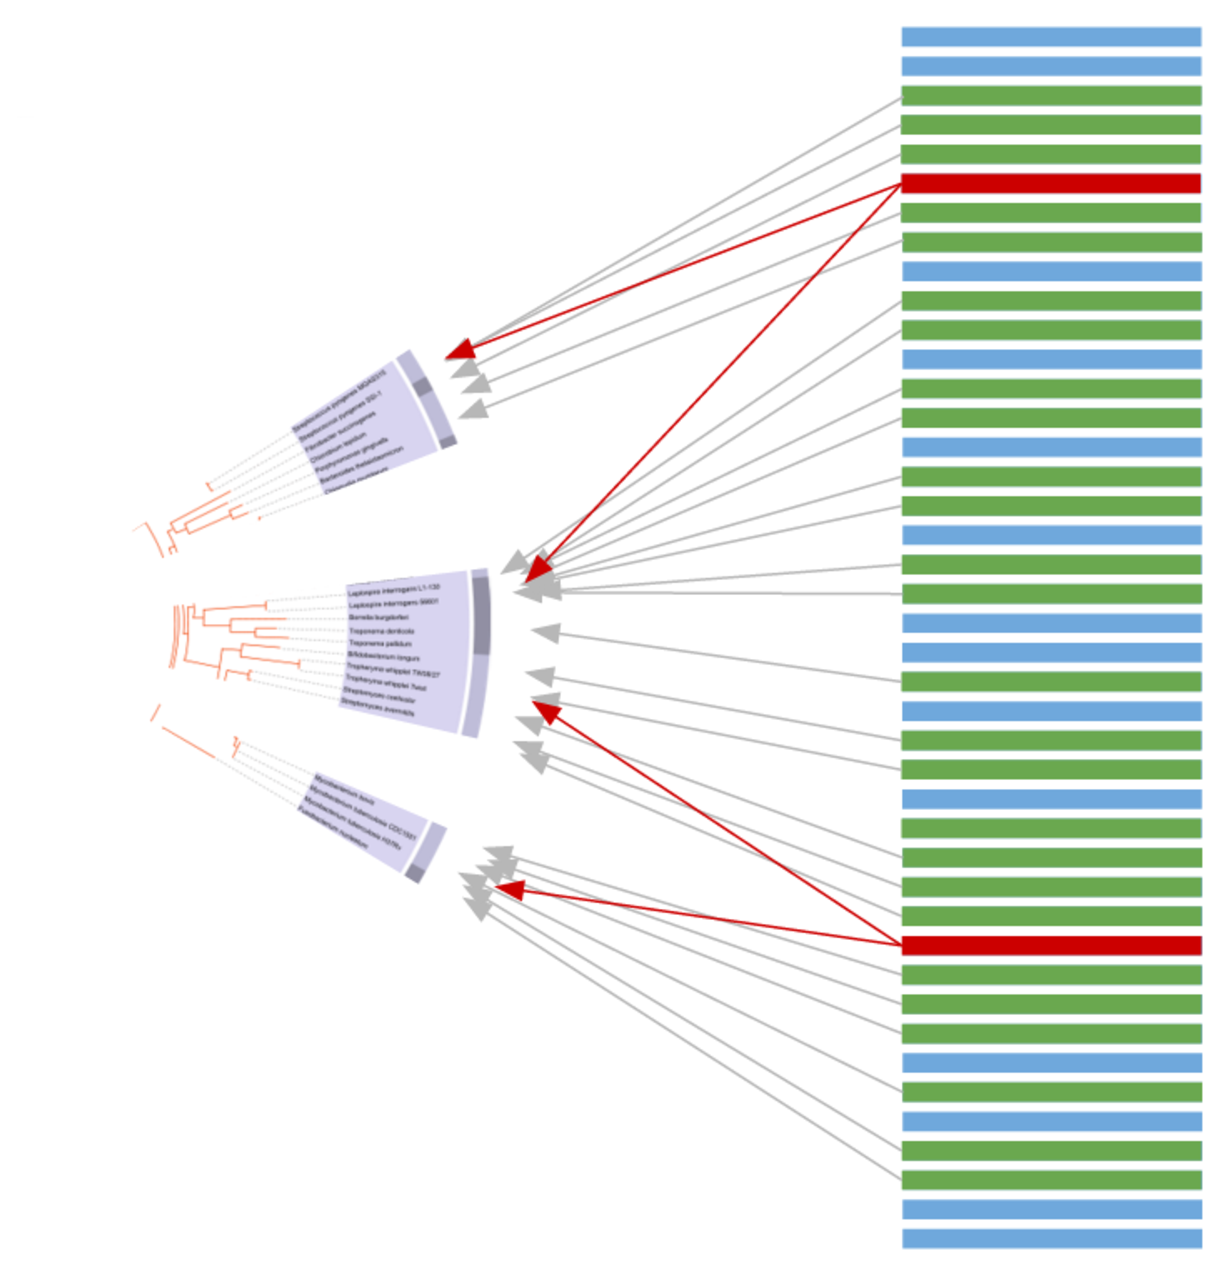
\includegraphics[width=0.54\linewidth, right]{assets/Subset}
        \end{block}
        \begin{block}{Making Sense of the Results}
        \includegraphics[width=1\linewidth]{assets/coverage_plot_good}\newline\newline
        \includegraphics[width=1\linewidth]{assets/coverage_plot_bad}\newline\newline
        \end{block}

    \end{column}

    %%%%%%%%%%%%%%%%%%%%%%%%%%%%%%%

    \begin{column}{.3\linewidth}
        \begin{block}{Architecture}
            A computational pipeline in YAX is\\
            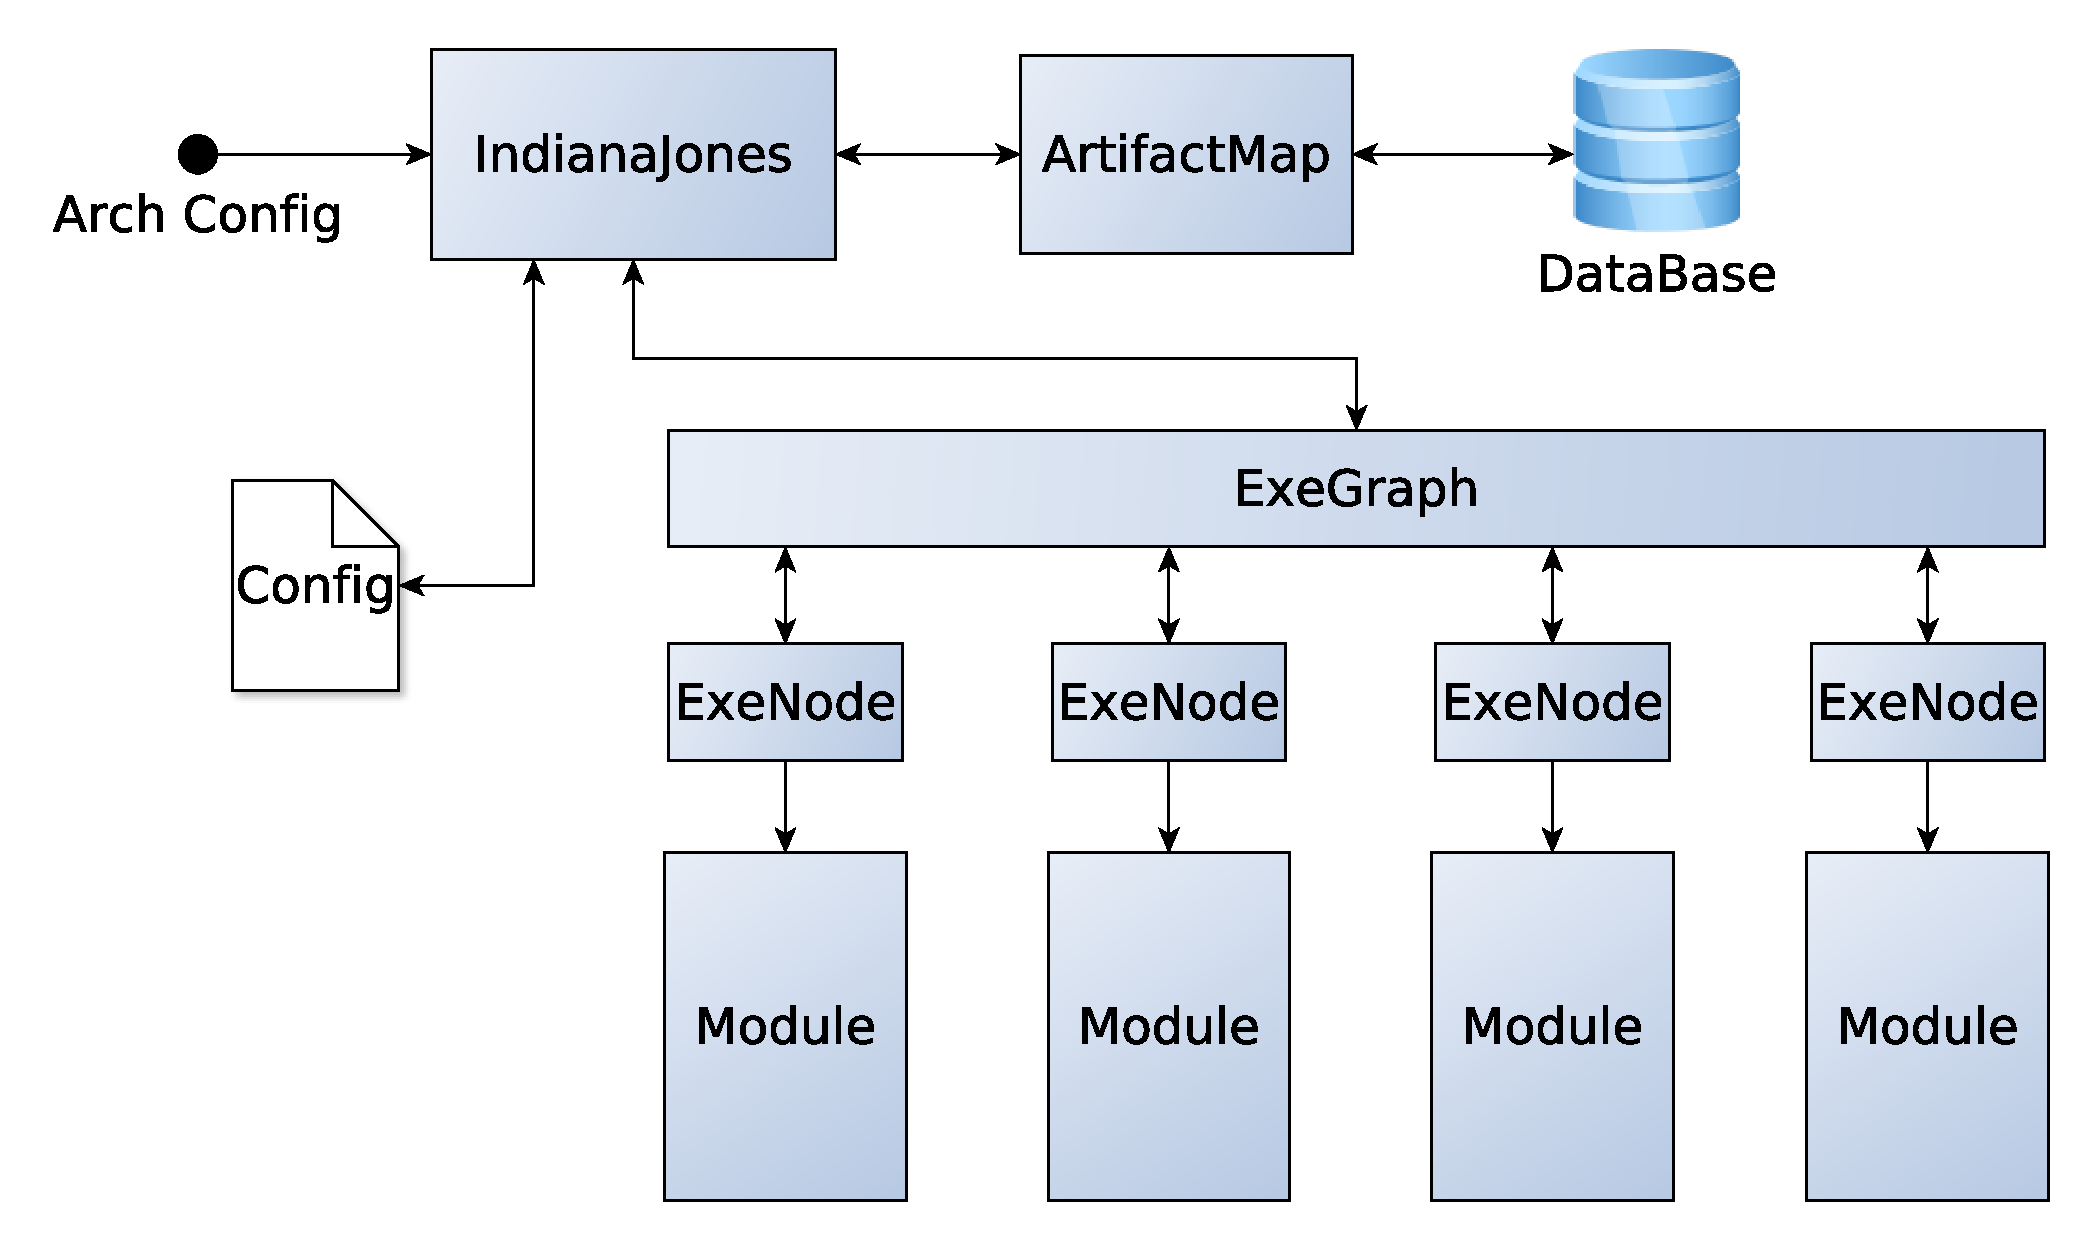
\includegraphics[width=1\linewidth]{assets/arch}\newline\newline

        \end{block}
        \begin{block}{Outcomes}
            YAX is designed to be highly modular and capable of adapting along side technological developments. As part of its development
            YAX was built to not only provide one solution but to investigate a number of possible solutions. The near future of YAX will
            see new modules developed to make fool use of its flexibility.

        \end{block}
        \begin{block}{Future Work}
            YAX is designed to be highly modular and capable of adapting along side technological developments. As part of its development
            YAX was built to not only provide one solution but to investigate a number of possible solutions. The near future of YAX will
            see new modules developed to make fool use of its flexibility.

        \end{block}

        %%%%%%%%%%%%%%%%%%%%%%%%%%%%%%%%%%%%%%%%%%%%%%%%%%%%%%%%%%%%%%%%%%%%%%%%%%%%%%%%%%%%%%%%%%%%%%%%%%%%%%%%%%%%



%%%%%%%%%%%%%%%%%%%%%%%%%%%%%%%%%%%%%%%%%%%%%%%%%%%%%%%

    \end{column}
  \end{columns}

\end{frame}

\end{document}


%%%%%%%%%%%%%%%%%%%%%%%%%%%%%%%%%%%%%%%%%%%%%%%%%%%%%%%%%%%%%%%%%%%%%%%%%%%%%%%%%%%%%%%%%%%%%%%%%%%%
%%% Local Variables:
%%% mode: latex
%%% TeX-PDF-mode: t
%%% End:
